\documentclass{article}
%-------------------------------------------------------
\usepackage{graphicx}
\usepackage{subcaption}
\usepackage{amsmath}
%-------------------------------------------------------
\begin{document}
%-------------------------------------------------------
\title{Flyback Converter Design and Analysis}
\author{Mohamed Gueni}
\date{\today}
%-------------------------------------------------------
\maketitle
%-------------------------------------------------------
\tableofcontents
%-------------------------------------------------------

\section{Introduction}
A flyback converter is a type of DC-DC converter widely used in applications requiring a single output voltage and galvanic isolation between input and output. This document details the design of a single-output flyback converter with a 3-36V DC input (nominal 24V DC) and a 12V DC output, capable of delivering up to 2A. The converter includes an RC snubber and an RCD clamp to handle switching transients and protect the components.

\section{System Diagram}
%-------------------------------------------------------
\begin{figure}[htbp]
    \centering
    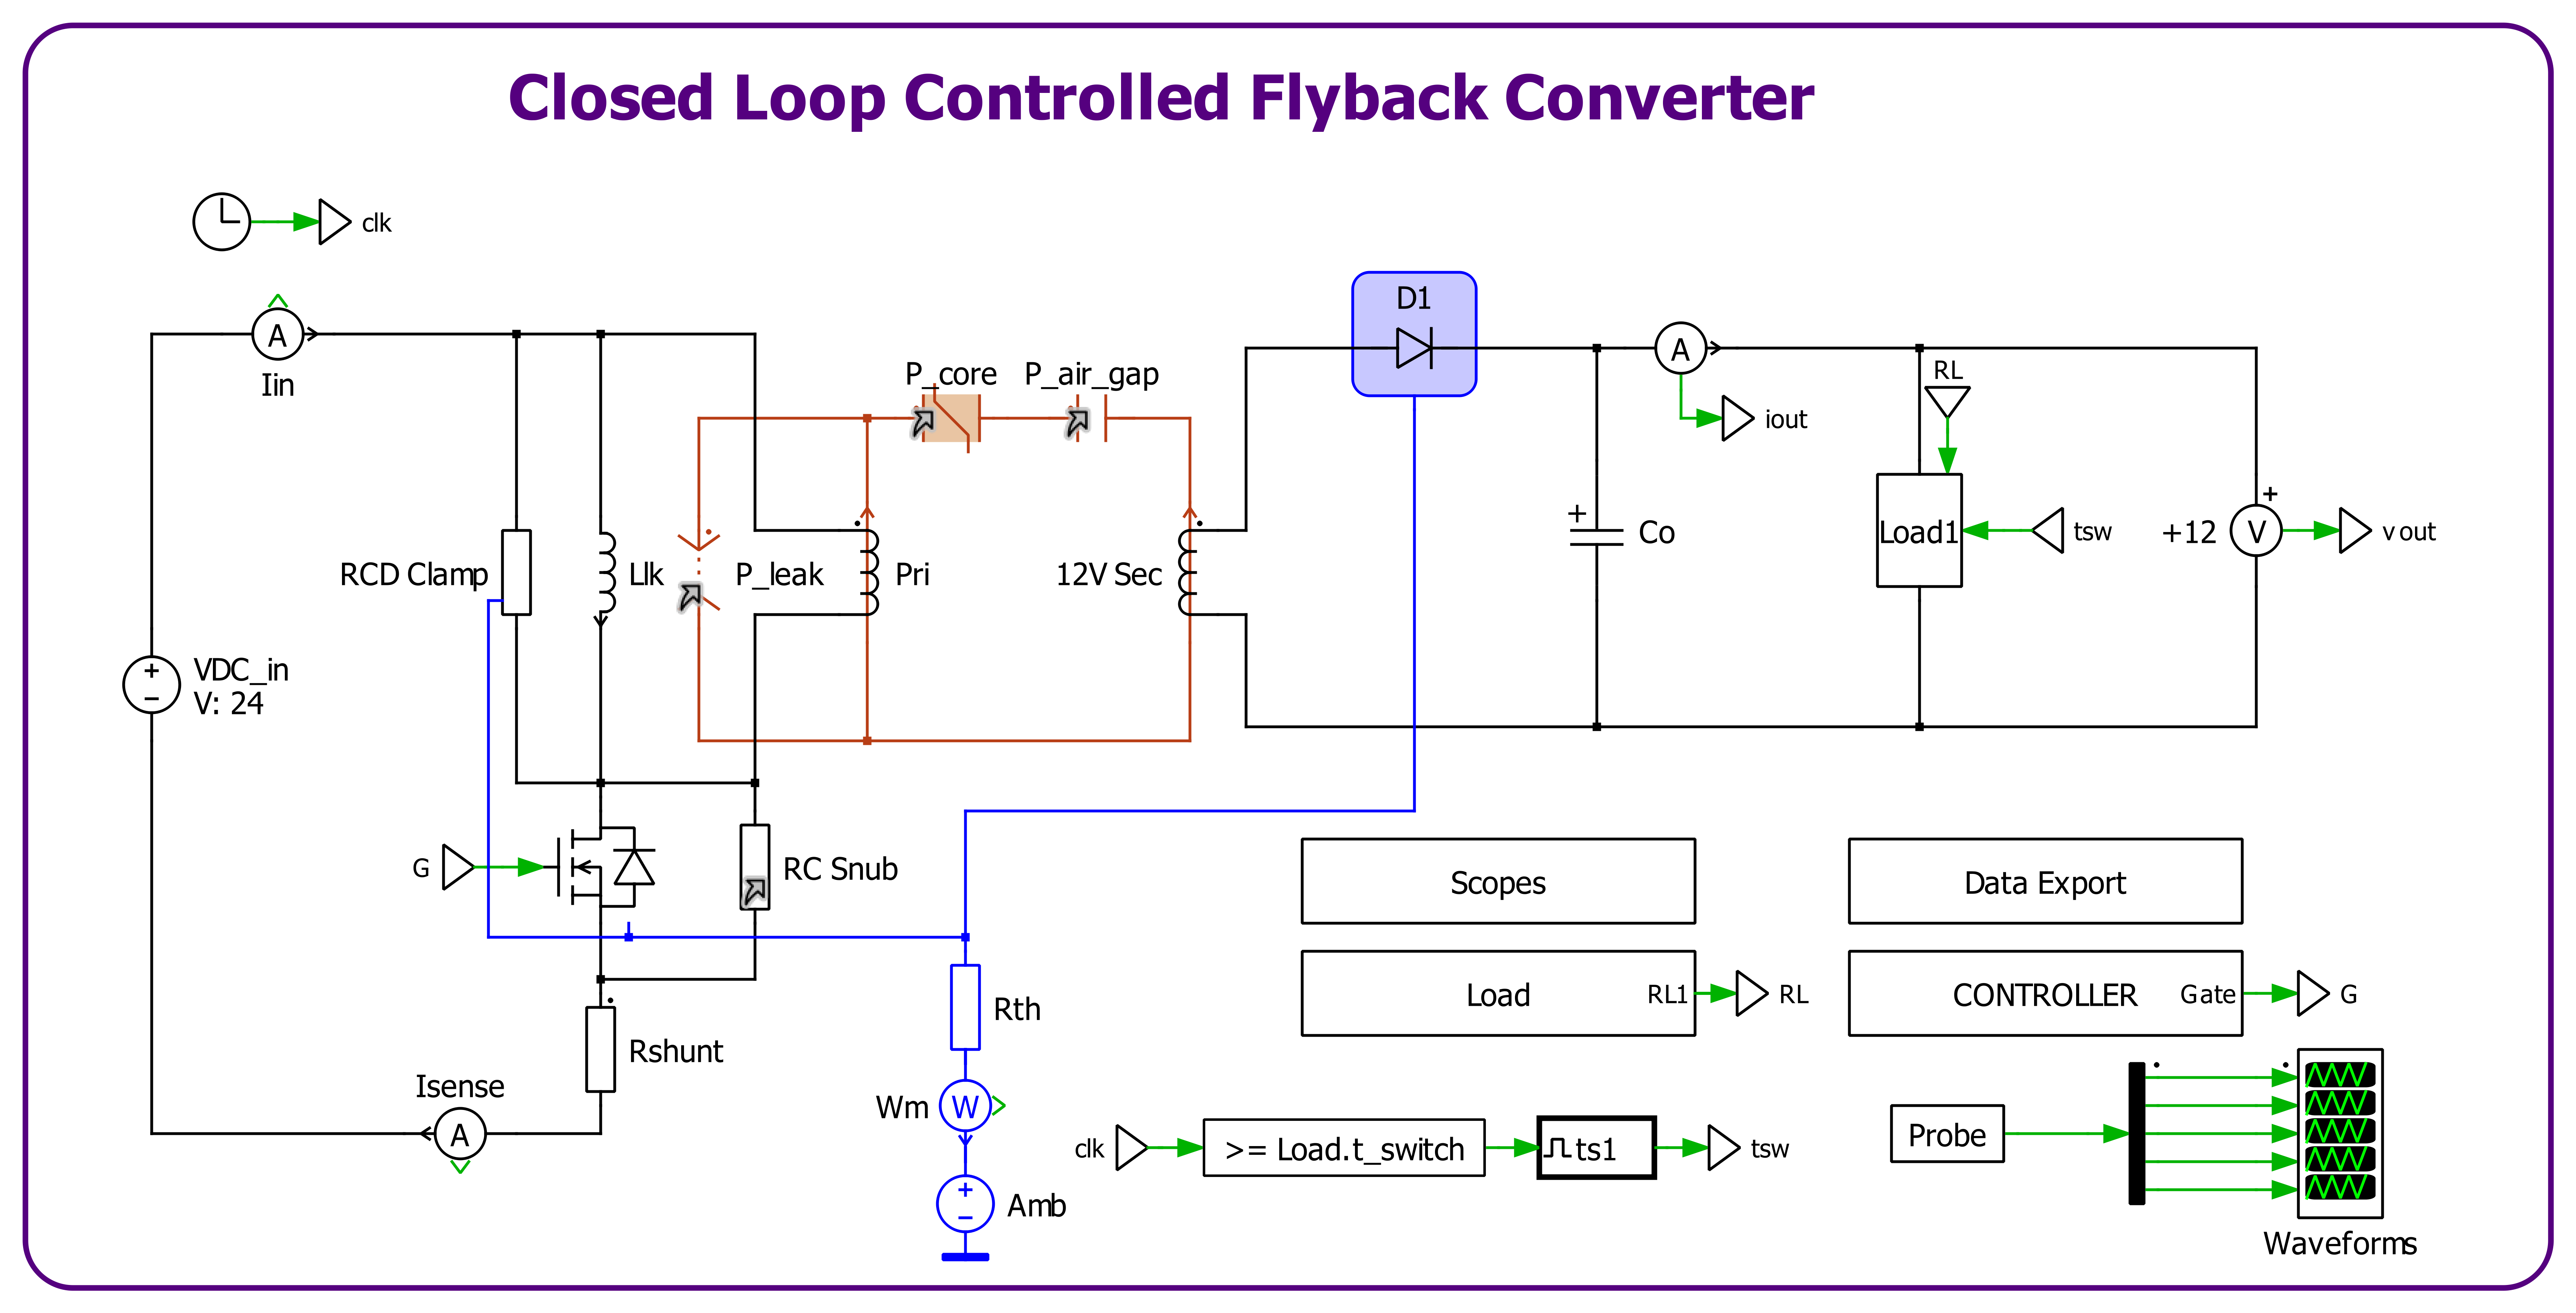
\includegraphics[width=\textwidth]{flyback.jpg}
    \caption{Flyback Converter System Diagram}
    \label{fig:Flyback}
\end{figure}
%-------------------------------------------------------

\section{System Description}
The flyback converter operates by storing energy in a transformer during the switch-on period and releasing it to the output during the switch-off period. This section elaborates on each part of the system.

\subsection{Transformer}
The transformer in a flyback converter serves two primary purposes:
\begin{itemize}
    \item \textbf{Energy Storage and Transfer}: During the switch-on period, energy is stored in the transformer's magnetic field. During the switch-off period, this energy is transferred to the output.
    \item \textbf{Voltage Transformation and Isolation}: The transformer steps down the input voltage to the required output level and provides galvanic isolation between the input and the output.
\end{itemize}

\subsubsection{Turns Ratio Calculation}
The turns ratio is a key parameter that affects the output voltage. The given transformer has a turns ratio of 8:1:1 (primary:secondary:auxiliary). We can verify this based on the desired output voltage and duty cycle.

\[
\frac{N_{pri}}{N_{sec}} = \frac{V_{out} + V_{f}}{V_{in} \times D_{max}}
\]

Given data:
\begin{itemize}
    \item $V_{in}$ = 24V (nominal)
    \item $V_{out}$ = 12V
    \item $V_{f}$ = 0.5V (Schottky diode)
    \item $D_{max}$ = 0.5 (typical for flyback converters)
\end{itemize}

Substituting values:

\[
\frac{N_{pri}}{N_{sec}} = \frac{12V + 0.5V}{24V \times 0.5} = \frac{12.5V}{12V} = 1.04
\]
:1:1 ratio of the chosen transformer provides a margin to accommodate variations in input voltage if we need it to.

\subsubsection{Primary Inductance}
The primary inductance $L_{pri}$ is crucial for determining the converter’s mode of operation. For continuous conduction mode (CCM), $L_{pri}$ must be sufficiently large.

\[
L_{pri} = \frac{V_{in} \times D_{max} \times (1 - D_{max})}{f_s \times I_{pri, peak}}
\]

Given:
\begin{itemize}
    \item $V_{in}$ = 24V (nominal)
    \item $D_{max}$ = 0.5
    \item $f_s$ = 100 kHz
    \item $I_{pri, peak}$ is determined by the maximum output power and efficiency. Assuming 85\% efficiency, and a maximum output power of $P_{out} = V_{out} \times I_{out} = 12V \times 2A = 24W$:
    \[
    I_{pri, peak} = \frac{P_{out}}{\eta \times V_{in}} = \frac{24W}{0.85 \times 24V} \approx 1.18A
    \]
\end{itemize}

Substituting the values:

\[
L_{pri} = \frac{24V \times 0.5 \times (1 - 0.5)}{100 \times 10^3 \times 1.18A} = \frac{6V}{118 \times 10^3} \approx 50.85\ \mu H
\]

Since the actual transformer has a primary inductance of 670 µH, it will operate in continuous conduction mode.

\subsection{Output Rectification and Filtering}
The output rectification and filtering stages convert the AC voltage from the transformer's secondary winding into DC voltage and reduce voltage ripple.

\subsubsection{Output Capacitor}
The capacitor filters the rectified voltage to reduce ripple and provide a stable DC output.

\[
C_{out} = \frac{I_{out} \times D_{max}}{f_s \times \Delta V_{out}}
\]

Given:
\begin{itemize}
    \item $I_{out}$ = 2A
    \item $D_{max}$ = 0.5
    \item $f_s$ = 100 kHz
    \item $\Delta V_{out}$ = 0.1V (desired ripple)
\end{itemize}

Substituting the values:

\[
C_{out} = \frac{2A \times 0.5}{100 \times 10^3 \times 0.1V} = \frac{1A}{10V} = 100\ \mu F
\]

The output capacitor should be rated at least 100 µF with a voltage rating above the output voltage.

\subsection{RC Snubber Circuit}
The RC snubber circuit is used to dampen oscillations caused by the transformer's leakage inductance during the switching transitions.

\subsection{RC Snubber Circuit Calculation}
The RC snubber circuit is designed to dampen the oscillations caused by the transformer's leakage inductance during the switching transitions. Given:

\[
R_s = 1 \, k\Omega, \quad L_{leak} = 8 \, \mu H
\]

\subsubsection{Snubber Capacitor Calculation}
The snubber capacitor \( C_s \) is calculated to critically dampen the oscillations. The value of \( C_s \) can be found using the following formula:

\[
C_s = \frac{1}{2 \pi f_{ring} R_s}
\]

Where:
\begin{itemize}
    \item \( f_{ring} \) is the ringing frequency, typically a few MHz. Let's assume \( f_{ring} = 2 \, MHz \).
\end{itemize}

Substituting the values:

\[
C_s = \frac{1}{2 \pi \times 2 \times 10^6 \times 1 \times 10^3} \approx 79.6 \, pF
\]

Therefore, the snubber capacitor \( C_s \) should be approximately \( 79.6 \, pF \).

\subsubsection{Verification of Snubber Resistor Selection}
The resistor \( R_s \) was chosen as \( 1 \, k\Omega \). We can verify its suitability using the following relation:

\[
R_s = \sqrt{\frac{L_{leak}}{C_s}}
\]

Substituting the values:

\[
R_s = \sqrt{\frac{8 \times 10^{-6}}{79.6 \times 10^{-12}}} \approx 10 \, k\Omega
\]

Since the calculated \( R_s \) is \( 10 \, k\Omega \) but we selected \( 1 \, k\Omega \), this indicates that the circuit will be underdamped, which might allow for some oscillations. However, this choice can still be acceptable if the damping is sufficient for the application's EMI requirements.

\subsubsection{Final Snubber Component Values}
Given the practical considerations and typical design trade-offs, the selected components for the RC snubber are:

\[
R_s = 1 \, k\Omega, \quad C_s \approx 79.6 \, pF
\]

These values are chosen to balance damping efficiency with component sizes and costs.

\subsection{RCD Clamp Circuit Calculation}
The RCD (Resistor-Capacitor-Diode) clamp circuit is designed to limit the peak voltage across the MOSFET by diverting excess energy stored in the transformer's leakage inductance. Given:

\[
R_{clamp} = 100 \, k\Omega, \quad L_{leak} = 8 \, \mu H
\]

\subsubsection{Clamp Resistor Calculation}
The clamp resistor \( R_{clamp} \) is chosen to dissipate the energy stored in the leakage inductance. The resistor value is given as \( 100 \, k\Omega \).

\subsubsection{Clamp Capacitor Calculation}
The clamp capacitor \( C_{clamp} \) stores the energy to limit the voltage spike across the MOSFET. The value of \( C_{clamp} \) can be calculated using the energy equation:

\[
\Delta E = \frac{1}{2} L_{leak} I_{peak}^2
\]

Where:
\begin{itemize}
    \item \( L_{leak} \) is the leakage inductance (\( 8 \, \mu H \)).
    \item \( I_{peak} \) is the peak current through the transformer.
\end{itemize}

Assuming a peak current \( I_{peak} \) based on the maximum input voltage (\( V_{in(max)} = 36 \, V \)) and maximum output current (\( I_{out(max)} = 2 \, A \)):

\[
I_{peak} = \frac{V_{in(max)}}{R_{clamp}} = \frac{36 \, V}{100 \times 10^3 \, \Omega} = 0.36 \, mA
\]

Now, calculate the energy stored in the leakage inductance:

\[
\Delta E = \frac{1}{2} \times 8 \times 10^{-6} \, H \times (0.36 \times 10^{-3} \, A)^2 \approx 5.18 \times 10^{-13} \, J
\]

The clamp capacitor \( C_{clamp} \) can be found using:

\[
C_{clamp} = \frac{2 \Delta E}{\Delta V_{clamp}^2}
\]

Where \( \Delta V_{clamp} \) is the allowable voltage ripple across the clamp capacitor. Assuming \( \Delta V_{clamp} = 1 \, V \):

\[
C_{clamp} = \frac{2 \times 5.18 \times 10^{-13} \, J}{(1 \, V)^2} \approx 1.04 \, pF
\]
\subsubsection{Clamp Resistor}
The resistor \( R_{clamp} \) is chosen to dissipate the energy stored in the leakage inductance, and its value is \( 100 \, k\Omega \).

\subsubsection{Clamp Capacitor}
The capacitor \( C_{clamp} \) is selected to store the energy and limit the voltage spike across the MOSFET. The chosen value is \( 0.1 \, \mu F \).

\subsubsection{Practical Considerations}
While theoretical calculations can provide a starting point, the chosen values of \( R_{clamp} = 100 \, k\Omega \) and \( C_{clamp} = 0.1 \, \mu F \) are practical and commonly used in RCD clamp circuits for flyback converters. These values are selected to ensure effective clamping, while also considering component availability and typical design practices.

The \( 0.1 \, \mu F \) capacitor ensures that the voltage spike across the MOSFET is sufficiently limited, and the \( 100 \, k\Omega \) resistor dissipates the energy at a rate that balances protection with efficiency.
These values are chosen to effectively limit the voltage spike across the MOSFET while ensuring that the energy stored in the leakage inductance is dissipated safely.



\section*{Reverse Polarity Protection}

When the input is connected correctly (positive to the source of the PMOS and negative to the drain), the PMOS will be in the ON state, allowing current to flow.

%-------------------------------------------------------
\begin{figure}[htbp]
    \centering
    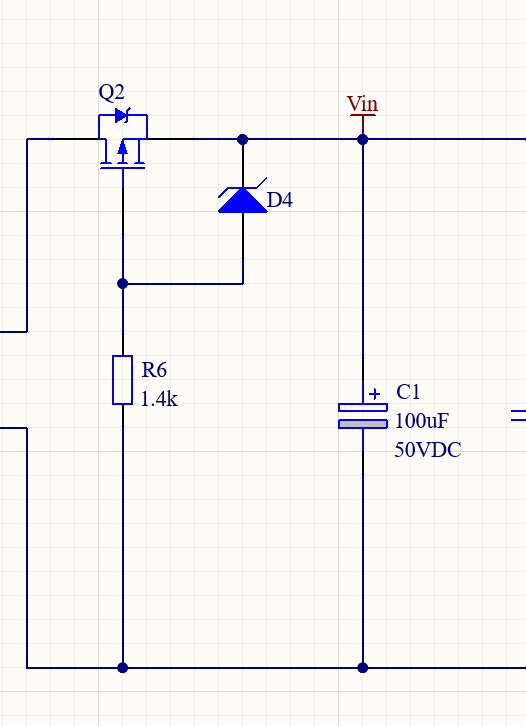
\includegraphics[width=\textwidth]{RVP.png}
    \caption{Reverse Polarity Protection}
    \label{fig:RVP}
\end{figure}
%-------------------------------------------------------
 If the polarity is reversed, the PMOS remains OFF, preventing current from flowing and protecting your circuit
\section*{Reverse Polarity Protection (Continued)}
\subsection*{1. Selecting the PMOS Transistor}

\begin{itemize}
    \item \textbf{Voltage Rating (V\(_{DS}\)):} The PMOS should have a drain-source voltage rating higher than the maximum input voltage. Since the input can go up to 36V, a PMOS with at least a 40V V\(_{DS}\) rating is recommended to provide a margin.
    
    \item \textbf{Current Rating (I\(_{D}\)):} The PMOS must handle the maximum current drawn by your circuit. Since the circuit could draw up to 2A, we choose a PMOS with a current rating higher than 2A, preferably 5A or more for safety.
    
    \item \textbf{R\(_{DS(on)}\):} This is the on-state resistance of the PMOS when it's fully turned on. Lower R\(_{DS(on)}\) values reduce power loss and heat dissipation. A PMOS with R\(_{DS(on)}\) in the range of a few milliohms (m\(\Omega\)) is suitable.
\end{itemize}

\subsection*{2. Selecting the Zener Diode}

\begin{itemize}
    \item \textbf{Zener Voltage (V\(_Z\)):} The Zener diode ensures that the gate-source voltage (V\(_{GS}\)) of the PMOS stays within safe limits. We select a Zener voltage slightly higher than the PMOS gate threshold voltage (V\(_{GS(th)}\)) but lower than the maximum allowed V\(_{GS}\) for the PMOS.
    
    \item \textbf{For example:} If the PMOS has a V\(_{GS(th)}\) of -2V and a maximum V\(_{GS}\) of -20V, we could choose a Zener diode with a V\(_Z\) of 10V. This ensures the gate is clamped to a voltage that fully turns on the PMOS but doesn’t exceed the maximum V\(_{GS}\).
\end{itemize}

\subsection*{3. Selecting the Resistor}

\begin{itemize}
    \item \textbf{Resistor Value (R):} The resistor limits the current flowing through the Zener diode and ensures that the PMOS gate is pulled to the source (ground) when the input is connected with the correct polarity.
    
    \item \textbf{Calculation:} The resistor value can be calculated using Ohm's Law:
    \[
    R = \frac{V_{in} - V_{Z}}{I_{Z}}
    \]
    Where \(V_{in}\) is the input voltage, \(V_{Z}\) is the Zener voltage, and \(I_{Z}\) is the Zener current, which should be enough to activate the Zener diode but not too high to damage it (typically in the range of 5-20mA).
    
    \item \textbf{Example:} For a Zener diode with a 10V rating and a desired current of 10mA, with an input voltage of 24V:
    \[
    R = \frac{24V - 10V}{10mA} = 1.4k\Omega
    \]
    A resistor of approximately 1.4k\(\Omega\) should be used.
\end{itemize}


\section{MOSFET Model Testing in PLECS}

The objective of this project includes testing a MOSFET model developed in PLECS software. This section describes the approach used to validate the MOSFET model through simulation, ensuring its accuracy and performance in the flyback converter circuit.

\subsection{Simulation Setup}
To test the MOSFET model, a detailed simulation setup was created in PLECS. The setup includes:

\begin{itemize}
    \item **Flyback Converter Circuit:** The MOSFET model is integrated into the flyback converter circuit designed with parameters specified in previous sections.
    \item **Input and Output Conditions:** The simulation conditions match the real-world operating conditions of the converter, including varying input voltages and load conditions.
    \item **Component Models:** All components, including the MOSFET, transformer, diodes, and capacitors, are modeled accurately to reflect their real-life behavior.
\end{itemize}

\subsection{Simulation Objectives}
The primary objectives of the simulation are:

\begin{itemize}
    \item **Verify MOSFET Performance:** Ensure that the MOSFET operates correctly within the specified voltage and current ranges, and meets the design requirements.
    \item **Analyze Switching Behavior:** Evaluate the switching performance of the MOSFET, including turn-on and turn-off times, and the impact on the overall converter efficiency.
    \item **Assess Thermal Performance:** Check the thermal performance of the MOSFET under different operating conditions to ensure it remains within safe temperature limits.
\end{itemize}

\subsection{Simulation Results}
The results of the simulation will be presented and analyzed in subsequent sections. Figures and plots will include:

\begin{itemize}
    \item **Voltage and Current Waveforms:** Displaying the MOSFET's drain-source voltage, gate-source voltage, and current waveforms.
    \item **Efficiency and Losses:** Analyzing the efficiency of the flyback converter and the losses associated with the MOSFET.
    \item **Thermal Analysis:** Showing the temperature distribution and thermal performance of the MOSFET.
\end{itemize}

\subsection{Figures and Analysis}
Figures illustrating the simulation results will be added here. Each figure will be accompanied by a detailed analysis of the MOSFET's performance, including comparisons with expected behavior and design specifications.

% Placeholder for figures
% \begin{figure}[htbp]
%     \centering
%     \includegraphics[width=\textwidth]{mosfet_simulation_results.png}
%     \caption{MOSFET Simulation Results}
%     \label{fig:MOSFET_Simulation}
% \end{figure}






















\section{References}

\begin{enumerate}
    \item R. W. Erickson, \textit{Fundamentals of Power Electronics}, New York: Chapman \& Hall, 1997.
\end{enumerate}

\section{Units}

\begin{enumerate}
    \item Farads (\textbf{F}).................: Unit of capacitance.
    \item Amps (\textbf{A})..................: Unit of electric current.
    \item Volts (\textbf{V})...................: Unit of electric potential.
    \item Ohms (\textbf{$\Omega$})............: Unit of electrical resistance.
    \item Henrys (\textbf{H}).................: Unit of inductance.
    \item Watts (\textbf{W}).................: Unit of power.
    \item Hertz (\textbf{Hz}).................: Unit of frequency.
    \item Teslas (\textbf{T})...................: Unit of magnetic flux density.
    \item Webers (\textbf{Wb}).............: Unit of magnetic flux.
    \item Decibels (\textbf{dB}).............: Unit of measurement for the power level of an electrical signal.
\end{enumerate}

%-------------------------------------------------------
\end{document}
%-------------------------------------------------------

